\documentclass[DaoFP]{subfiles}
\begin{document}
\setcounter{chapter}{19}

\chapter{Kan 扩张}

如果范畴论不断提高抽象层次,那是因为它致力于发现模式。一旦模式被发现,就该研究这些模式形成的模式,依此类推。

我们已经在越来越高的抽象层次上看到了相同的反复出现的概念,并且描述得越来越简洁。

例如,我们首先使用泛构造定义了积。然后我们看到积定义中的跨度是自然变换。这导致将积解释为极限。接着我们看到可以使用伴随来定义它。我们能够将其与余积结合在一个简洁的公式中:
\[ (+) \dashv \Delta \dashv (\times) \]
老子说:“欲缩之,必固张之。”

Kan 扩张将抽象层次提得更高。Mac Lane 说:“所有概念都是 Kan 扩张。”

\section{闭幺半范畴}

我们已经看到如何将函数对象定义为范畴积的右伴随:
\[ \cat C (a \times b, c) \cong \cat C (a, [b, c]) \]
这里我使用了替代符号 $[b, c]$ 表示内部 hom——即指数 $c^b$。

两个函子之间的伴随关系可以被认为是一个是另一个的伪逆。它们不组合成恒等函子,但它们的组合通过单位和余单位与恒等函子相关。例如,如果你仔细观察,柯里化伴随的余单位:
\[ \varepsilon_{b c} \colon [b, c] \times b \to c \]
暗示着 $[b, c]$ 在某种意义上体现了乘法的逆。它在以下公式中扮演着与 $c/b$ 类似的角色:
\[ c/b \times b = c \]

以典型的范畴论方式,我们可能会问:如果我们用其他东西替换积会怎样?显然,用余积替换它不起作用(因此我们没有减法的类比)。但也许还有其他表现良好的二元运算具有右伴随。

推广积的自然设置是具有张量积 $\otimes$ 和单位对象 $I$ 的幺半范畴。如果我们有一个伴随:
\[ \cat C (a \otimes b, c) \cong \cat C (a, [b, c]) \]
我们将该范畴称为\emph{闭幺半范畴}。在典型的范畴论符号滥用中,除非引起混淆,我们将使用与笛卡尔 hom 相同的符号(一对方括号)来表示幺半内部 hom。张量积的右伴随还有一种替代的\index{棒棒糖}棒棒糖符号:
\[ \cat C (a \otimes b, c) \cong \cat C (a, b \multimap c) \]
它经常在\index{线性类型}线性类型的上下文中使用。

内部 hom 的定义在对称幺半范畴中表现良好。如果张量积不是对称的,伴随关系定义了一个\emph{左闭}幺半范畴。左内部 hom 是“后乘”函子 $(- \otimes b)$ 的伴随。右闭结构定义为“前乘”函子 $(b \otimes -)$ 的右伴随。如果两者都定义了,则该范畴称为\index{双闭幺半范畴}\emph{双闭}。

\subsection{Day 卷积的内部 hom}

作为一个例子,考虑在余预层范畴中具有 Day 卷积的对称幺半结构:
\[ (F \star G) x = \int^{a, b} \cat C (a \otimes b, x) \times F a \times G b \]
我们寻找伴随:
\[ [\cat C, \Set] (F \star G, H) \cong  [\cat C, \Set] (F, [G, H]_{\text{Day}}) \]
左侧的自然变换可以写成关于 $x$ 的 end:
\[ \int_x \Set \big( \int^{a, b} \cat C (a \otimes b, x) \times F a \times G b, H x \big) \]
我们可以使用共连续性将 coends 拉出:
\[ \int_{x, a, b} \Set \big( \cat C (a \otimes b, x) \times F a \times G b, H x \big) \]
然后我们可以使用 $\Set$ 中的柯里化伴随(方括号表示 $\Set$ 中的内部 hom):
\[ \int_{x, a, b} \Set \big( F a, [\cat C (a \otimes b, x)  \times G b, H x] \big) \]
最后,我们使用 hom-set 的连续性将两个 ends 移到 hom-set 内部:
\[ \int_{a} \Set \big( F a, \int_{x, b} [\cat C (a \otimes b, x)  \times G b, H x] \big) \]
我们发现 Day 卷积的右伴随由下式给出:
\[ \big([G, H]_{\text{Day}}\big) a = \int_{x, b} \big[\cat C(a \otimes b, x), [G b, H x]\big] \cong \int_b [G b, H (a \otimes b)]\]
最后的变换是 $\Set$ 中 Yoneda 引理的应用。
\begin{exercise}
在 Haskell 中实现 Day 卷积的内部 hom。提示:使用类型别名。
\end{exercise}
\begin{exercise}
实现伴随的见证:
\begin{haskell}
ltor :: (forall a. Day f g a -> h a) -> (forall a. f a -> DayHom g h a)
rtol :: Functor h => 
  (forall a. f a -> DayHom g h a) -> (forall a. Day f g a -> h a)
\end{haskell}
\end{exercise}

\subsection{幂与余幂}

在集合范畴中,内部 hom(函数对象或指数)与外部 hom(两个对象之间的态射集)同构:
\[ C^B \cong Set(B, C) \]
因此,我们可以将 $\Set$ 中定义内部 hom 的柯里化伴随重写为:
\[ \Set (A \times B, C)  \cong \Set \big(A, \Set (B, C)\big) \]
我们可以将这种伴随关系推广到 $B$ 和 $C$ 不是集合而是某个范畴 $\cat C$ 中的对象的情况。任何范畴中的外部 hom 始终是一个集合。但左侧不再由积定义。相反,它定义了集合 $A$ 在对象 $b$ 上的作用:
\[ \cat C (A \cdot b, c) \cong \Set \big( A, \cat C (b, c)\big) \]
这被称为\index{余幂}\emph{余幂}。

你可以将这种作用视为将 $b$ 的 $A$ 个副本相加(取余积)。例如,如果 $A$ 是一个二元集 $\mathbf 2$,我们得到:
\[ \cat C (\mathbf 2 \cdot b, c) \cong \Set \big( \mathbf 2, \cat C (b, c)\big) \cong \cat C(b, c) \times \cat C(b, c) \cong \cat C(b + b, c) \]
换句话说,
\[ \mathbf 2 \cdot b \cong b + b \]
在这个意义上,余幂用迭代加法定义了乘法,就像我们在学校学到的那样。

如果我们将 $b$ 乘以 hom-set $\cat C (b, c)$ 并对 $b$ 取 coend,结果与 $c$ 同构:
\[ \cat \int^b C(b, c) \cdot b \cong c \]
确实,由于 Yoneda 引理,从任意 $x$ 到两侧的映射是同构的:
\[ \cat C \big( \int^b \cat C(b, c) \cdot b, x\big) \cong \int_b \Set \big( \cat C(b, c), \cat C (b, x)\big) \cong \cat C (c, x)\]

正如预期的那样,在 $\Set$ 中,余幂退化为笛卡尔积。
\[ \Set (A \cdot B, C) \cong \Set \big( A, \Set(B, C)\big) \cong \Set (A \times B, C) \]

同样,我们可以将幂表示为迭代乘法。我们使用相同的右侧,但这次我们使用映射入来定义\index{幂}\emph{幂}:
\[ \cat C (b, A \pitchfork c) \cong \Set  \big(A, \cat C(b, c)\big) \]
你可以将幂视为将 $c$ 的 $A$ 个副本相乘。确实,将 $A$ 替换为 $\mathbf 2$ 会得到:
\[ \cat C (b, \mathbf 2 \pitchfork c) \cong \Set  \big(\mathbf 2, \cat C(b, c)\big) \cong \cat C(b, c) \times \cat C(b, c) \cong \cat C (b, c \times c)\]
换句话说:
\[ \mathbf 2 \pitchfork c \cong c \times c \]
这是 $c^2$ 的一种花哨写法。

如果我们将 $c$ 乘以 hom-set $\cat C(c', c)$ 并对所有 $c$ 取 end,结果与 $c'$ 同构:
\[ \int_c \cat C (c', c) \pitchfork c \cong c' \]
这由 Yoneda 引理得出。确实,从任意 $x$ 到两侧的映射是同构的:
\[ \cat C \big(x, \int_c \cat C (c', c) \pitchfork c\big) \cong \int_c \Set \big( \cat C(c', c), \cat C(x, c)\big)  \cong \cat C (x, c') \]

在 $\Set$ 中,幂退化为指数,它与 hom-set 同构:
\[ A \pitchfork C \cong C^A \cong \Set (A, C) \]
这是积对称性的结果。
\[ \Set(B, A \pitchfork C) \cong \Set (A, \Set(B, C)) \cong \Set (A \times B, C) \]
\[ \cong \Set (B \times A, C) \cong \Set (B, \Set (A, C))\]

\section{函子的逆}

范畴论的一个方面是通过执行有损变换来丢弃信息;另一个方面是恢复丢失的信息。我们已经看到了用自由函子(遗忘函子的伴随函子)来弥补丢失数据的例子。Kan 扩展是另一个例子。两者都弥补了由不可逆函子丢失的数据。

函子可能不可逆的原因有两个。一个是它可能将多个对象或箭头映射到单个对象或箭头上。换句话说,它在对象或箭头上不是单射的。另一个原因是它的像可能不覆盖整个目标范畴。换句话说,它在对象或箭头上不是满射的。

例如,考虑一个伴随 $L \dashv R$。假设 $R$ 不是单射的,并且它将两个对象 $c$ 和 $c'$ 坍缩为单个对象 $d$
\begin{align*}
R c &= d \\
R c' &= d
\end{align*}
$L$ 无法撤销这一点。它不能同时将 $d$ 映射到 $c$ 和 $c'$。它最多只能将 $d$ 映射到一个“更一般”的对象 $L d$,该对象有箭头指向 $c$ 和 $c'$。这些箭头是定义伴随的余单位分量所必需的:
\begin{align*}
\varepsilon_c &\colon L d \to c
\\
\varepsilon_{c'} &\colon L d \to c'
\end{align*}
其中 $L d$ 既是 $L (R c)$ 也是 $L (R c')$
\[
 \begin{tikzcd} [row sep=0.5cm, column sep=1cm]
 L d
 \arrow[d, "\varepsilon_c"]
 \arrow[dd, bend right, "\varepsilon_{c'}"']
 \\
 c
 \arrow[rr, red, dashed, ""]
 && d
 \arrow[ull, blue, bend right, dashed, "L"']
 \\
 c'
 \arrow[urr, red, bend right, dashed, "R"]
  \end{tikzcd}
\]

此外,如果 $R$ 在对象上不是满射的,函子 $L$ 必须以某种方式在那些不在 $R$ 的像中的 $\cat D$ 的对象上定义。同样,单位和余单位的自然性将限制可能的选择,只要这些对象与 $R$ 的像之间有箭头连接。

显然,所有这些约束意味着伴随只能在非常特殊的情况下定义。

Kan 扩展甚至比伴随更弱。

如果伴随函子像逆一样工作,那么 Kan 扩展就像分数一样工作。

如果我们重新绘制定义伴随的余单位和单位的图表,这一点最为明显。在第一个图表中,$L$ 似乎扮演了 $1/R$ 的角色。在第二个图表中,$R$ 假装是 $1/L$。

\[
 \begin{tikzcd} [row sep=1cm, column sep=1cm]
 \cat C
 \arrow[rr, "\text{Id}", "" {name=ID, below} ]
 \arrow[d, bend right, "R"']
 && \cat C
 \\
 \cat D
  \arrow[urr, bend right, "L"']
 \arrow[Rightarrow, "\varepsilon",  to=ID]
 \end{tikzcd}
 \qquad
 \begin{tikzcd} [row sep=1cm, column sep=1cm]
 \cat D
 \arrow[rr, "\text{Id}", "" {name=ID, below} ]
 \arrow[d, bend right, "L"']
 && \cat D
 \\
 \cat C
  \arrow[urr, bend right, "R"']
 \arrow[Rightarrow, "\eta",  from=ID]
 \end{tikzcd}
\]

右 Kan 扩展 $\text{Ran}_P F$ 和左 Kan 扩展 $\text{Lan}_P F$ 通过将恒等函子替换为某个函子 $F \colon \cat E \to \cat C$ 来推广这些。Kan 扩展然后扮演分数 $F/P$ 的角色。从概念上讲,它们撤销 $P$ 的动作,然后执行 $F$ 的动作。

\[
 \begin{tikzcd} [row sep=1cm, column sep=1cm]
 \cat E
 \arrow[rr, "F", "" {name=ID, below} ]
 \arrow[d, bend right, "P"']
 && \cat C
 \\
 \cat B
  \arrow[urr, bend right, "\text{Ran}_P F"']
 \arrow[Rightarrow, "\varepsilon",  to=ID]
 \end{tikzcd}
 \qquad
 \begin{tikzcd} [row sep=1cm, column sep=1cm]
 \cat E
 \arrow[rr, "F", "" {name=ID, below} ]
 \arrow[d, bend right, "P"']
 && \cat C
 \\
 \cat B
  \arrow[urr, bend right, "\text{Lan}_P F"']
 \arrow[Rightarrow, "\eta",  from=ID]
 \end{tikzcd}
\]

就像伴随一样,“撤销”并不完全。复合 $\text{Ran}_P F \circ P$ 不会重现 $F$;相反,它通过称为余单位的自然变换 $\varepsilon$ 与 $F$ 相关。类似地,复合 $\text{Lan}_P F \circ P$ 通过单位 $\eta$ 与 $F$ 相关。

注意,$F$ 丢弃的信息越多,Kan 扩展“逆”函子 $P$ 就越容易。在某种意义上,它只需要“模 $F$”地逆 $P$。

以下是 Kan 扩展的直觉。我们从一个函子 $F$ 开始:
\[
 \begin{tikzcd} \cat E
 \arrow[r, "F"]
 & \cat C
  \end{tikzcd}
\]
有第二个函子 $P$ 将 $\cat E$ 压缩到另一个范畴 $\cat B$ 中。这可能是一个有损且非满射的嵌入。我们的任务是以某种方式 \emph{扩展} $F$ 的定义以覆盖整个 $\cat B$。

在理想情况下,我们希望以下图表交换:
\[
 \begin{tikzcd} \cat E
 \arrow[r, "F"]
 \arrow[d, "P"']
 & \cat C
 \\
 \cat B
\arrow[ur, "Kan_P F"']
  \end{tikzcd}
\]
但这将涉及函子的相等性,这是我们尽量避免的。

次好的选择是要求通过此图表的两个路径之间存在自然同构。但即便如此,似乎要求过高。因此,我们最终要求一个路径可以变形为另一个路径,这意味着它们之间存在一个单向的自然变换。这个变换的方向区分了右 Kan 扩展和左 Kan 扩展。


\section{右 Kan 扩展}

右 Kan 扩展是一个函子 $\text{Ran}_P F$,配备一个自然变换 $\varepsilon$,称为 Kan 扩展的余单位,定义为:
\[ \varepsilon \colon (\text{Ran}_P F) \circ P \to F\]
\[
 \begin{tikzcd} [row sep=1cm, column sep=1cm]
 \cat E
 \arrow[rr, "F", "" {name=ID, below} ]
 \arrow[d, bend right, "P"']
 && \cat C
 \\
 \cat B
  \arrow[urr, blue, bend right, "\text{Ran}_P F"']
 \arrow[Rightarrow, blue, "\varepsilon",  to=ID]
 \end{tikzcd}
\]

对 $(\text{Ran}_P F, \varepsilon)$ 是普遍(universal)的,即在所有这样的对 $(G, \alpha)$ 中,其中 $G$ 是一个函子 $G \colon \cat B \to \cat C$,而 $\alpha$ 是一个自然变换:
\[ \alpha \colon G \circ P \to F \]
\[
 \begin{tikzcd} [row sep=1cm, column sep=1cm]
 \cat E
 \arrow[rr, "F", "" {name=ID, below} ]
 \arrow[d, bend right, "P"']
 && \cat C
 \\
 \cat B
  \arrow[urr, red, bend right, "G"']
 \arrow[Rightarrow, red, "\alpha",  to=ID]
 \end{tikzcd}
\]

普遍性意味着对于任何这样的 $(G, \alpha)$,存在唯一的自然变换 $\sigma \colon G \to \text{Ran}_P F$
\[
\begin{tikzcd}[row sep=2cm, column sep=2cm]
\cat E  \ar[d, bend right, "P"', "" {name=P}]
            \ar[r, "F", ""  {name=F, below, near start, bend right}]
&
\cat C
\\
\cat B
    \ar[ur, red, bend left, "G", "" {name=G, below}]
    \ar[ur, blue, bend right, "\text{Ran}_P F"', "" {name=Ran}]
\arrow[Rightarrow, "\sigma", from=G, to=Ran]
\end{tikzcd}
\]
它将 $\alpha$ 分解,即:
\[ \alpha = \varepsilon \cdot (\sigma \circ P) \]
这是自然变换的垂直和水平组合,其中 $\sigma \circ P$ 是 $\sigma$ 的“whiskering”。以下是相同的方程用弦图表示:

\[
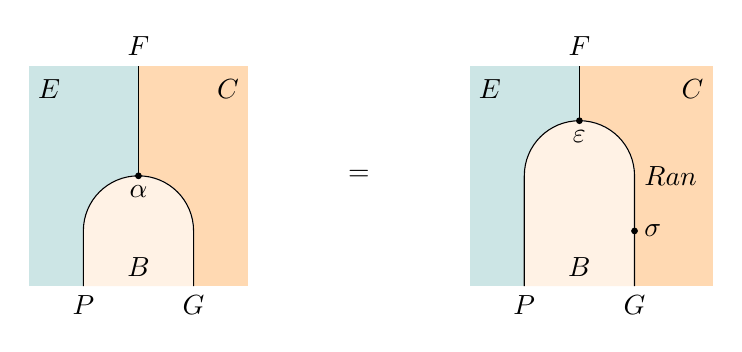
\begin{tikzpicture}
\def \dx {0.7}
\def \dy {0.7}

\def \xa{-3 * \dx};
\def \xb{-2 * \dx};
\def \xc{-1 * \dx};
\def \xd{0};
\def \xe{1 * \dx};

\def \ya{0};
\def \yb{1 * \dy};
\def \yc{2 * \dy};
\def \yd{3 * \dy};
\def \ye{4 * \dy};

% left background
\filldraw[fill=blue!50!green!20, draw=white] (\xa, \ye) rectangle (\xc, \ya);
% right background
\filldraw[fill=orange!30, draw=white] (\xc, \ye) rectangle (\xe, \ya);
% fill shape\yb
\path [fill=orange!10, draw=white]  (\xb, \ya) to (\xb, \yb) to [out=90, in=180]  (\xc, \yc) to  [out=0, in=90] (\xd, \yb) to (\xd, \ya);

% cup
\draw (\xb, \ya) to (\xb, \yb) to [out=90, in=180]  (\xc, \yc) to  [out=0, in=90] (\xd, \yb) to (\xd, \ya);
\draw (\xc, \yc) -- (\xc, \ye);

% natural transformations
\filldraw[black] (\xc, \yc) circle (1 pt);
\node [below] at (\xc, \yc) {$\alpha$};

% categories
\node[right] at (\xa, \ye - 0.3) {$\cat E$};
\node[left] at (\xe, \ye - 0.3) {$\cat C$};
\node[above] at (\xc, \ya) {$\cat B$};
% functors
\node [below] at (\xb, \ya) {$P$};
\node [below] at (\xd, \ya) {$G$};
\node [above] at (\xc, \ye) {$F$};

%-----------------
\node (eq) at (3 * \dx, \yc) {$=$};
% right diagram

\def \xa{5 * \dx};
\def \xb{6 * \dx};
\def \xc{7 * \dx};
\def \xd{8 * \dx};
\def \xe{9 * \dx + 0.3};

% left background
\filldraw[fill=blue!50!green!20, draw=white] (\xa, \ye) rectangle (\xc, \ya);
% right background
\filldraw[fill=orange!30, draw=white] (\xc, \ye) rectangle (\xe, \ya);
% fill shape
\path [fill=orange!10, draw=white]  (\xb, \ya) to (\xb, \yc) to [out=90, in=180]  (\xc, \yd) to  [out=0, in=90] (\xd, \yc) to (\xd, \ya);

% cup
\draw (\xb, \ya) to (\xb, \yc) to [out=90, in=180]  (\xc, \yd) to  [out=0, in=90] (\xd, \yc) to (\xd, \ya);
\draw (\xc, \yd) -- (\xc, \ye);

% natural transformations
\filldraw[black] (\xc, \yd) circle (1 pt);
\node [below] at (\xc, \yd) {$\varepsilon$};

\filldraw[black] (\xd, \yb) circle (1 pt);
\node [right] at (\xd, \yb) {$\sigma$};

% categories
\node[right] at (\xa, \ye - 0.3) {$\cat E$};
\node[left] at (\xe, \ye - 0.3) {$\cat C$};
\node[above] at (\xc, \ya) {$\cat B$};
% functors
\node [below] at (\xb, \ya) {$P$};
\node [below] at (\xd, \ya) {$G$};
\node [above] at (\xc, \ye) {$F$};
\node [right] at (\xd, \yc) {$\text{Ran}$};

\end{tikzpicture}
\]

如果对于每个函子 $F$,沿 $P$ 的右 Kan 扩展都存在,那么普遍构造可以推广为一个伴随(adjunction)——这次是两个函子范畴之间的伴随:
\[ [\cat E, \cat C](G \circ P, F) \cong [\cat B, \cat C](G, \text{Ran}_P F) \]
对于每个属于左侧的 $\alpha$,存在一个唯一的属于右侧的 $\sigma$。

换句话说,如果对于每个 $F$,右 Kan 扩展都存在,那么它是函子预组合的右伴随:
\[ (- \circ P) \dashv \text{Ran}_P \]
这个伴随的余单位在 $F$ 处的分量是 $\varepsilon$。

这让人联想到柯里化(currying)伴随:
\[ \cat E (a \times b, c) \cong \cat E (a, [b, c]) \]
其中乘积被函子组合所取代。(这个类比并不完美,因为组合只有在自函子范畴中才能被视为张量积。)

\subsection{右 Kan 扩展作为 end}

回忆一下“忍者”Yoneda 引理:
\[ F b \cong \int_{e} \mathbf{Set} (\cat B(b, e), F e) \]
这里,$F$ 是一个余预层(co-presheaf),即从 $\cat B$ 到 $\Set$ 的函子。$F$ 沿 $P$ 的右 Kan 扩展推广了这个公式:
\[ (\text{Ran}_P F) b \cong \int_e \Set \big( \cat B (b, P e), F e\big) \]

这适用于余预层。通常我们感兴趣的是 $F \colon \cat E \to \cat C$,所以我们需要用 \index{幂}幂(power)替换 $\Set$ 中的 hom-集。因此,右 Kan 扩展由以下 end 给出(如果存在):
 \[ (\text{Ran}_P F) b \cong \int_e \cat B (b, P e) \pitchfork F e \]
 
 证明基本上是自明的:在每一步中只有一件事可做。我们从伴随开始:
  \[ [\cat E, \cat C](G \circ P, F) \cong [\cat B, \cat C](G, \text{Ran}_P F) \]
并用 end 重写它:
 \[ \int_e \cat C \big(G ( P e), F e\big) \cong \int_b \cat C\big(G b, (\text{Ran}_P F) b\big) \]
我们代入公式得到:
 \[ \cong  \int_b \cat C\big(G b,\int_e \cat B (b, P e) \pitchfork F e \big)\]
我们利用 hom-函子的连续性将 end 提到前面:
\[  \cong  \int_b \int_e \cat C\big(G b, \cat B (b, P e) \pitchfork F e \big) \]
然后我们使用幂的定义:
\[ \int_b \int_e \Set \big(  \cat B (b, P e), \cat C (G b, F e) \big) \]
并应用 Yoneda 引理:
\[ \int_e  \cat C \big(G (P e), F e\big) \]
这个结果确实是伴随的左侧。
 
如果 $F$ 是一个余预层,右 Kan 扩展公式中的幂退化为指数/hom-集:
  \[ (\text{Ran}_P F) b \cong \int_e \Set \big( \cat B (b, P e), F e\big) \]
 
 还要注意,如果 $P$ 有一个左伴随,我们称之为 $P^{-1}$,即:
 \[ \cat B(b, P e) \cong \cat E(P^{-1} b, e) \]
 我们可以使用“忍者”Yoneda 引理来评估 end:
 \[ (\text{Ran}_P F) b \cong \int_e \Set \big( \cat B (b, P e), F e\big) \cong \int_e \Set(\cat E(P^{-1} b, e), F e) \cong F(P^{-1} b)\]
得到:
 \[  \text{Ran}_P F \cong F \circ P^{-1} \]
 由于伴随是逆概念的弱化,这个结果与 Kan 扩展“反转” $P$ 并随后应用 $F$ 的直觉是一致的。
 
\subsection{Haskell 中的右 Kan 扩展}
右 Kan 扩展的 end 公式可以立即翻译为 Haskell 代码:
\begin{haskell}
newtype Ran p f b = Ran (forall e. (b -> p e) -> f e)
\end{haskell}

右 Kan 扩展的余单位 $\varepsilon$ 是一个从 \hask{(Ran p f)} 与 \hask{p} 的复合到 \hask{f} 的自然变换:
\begin{haskell}
counit :: forall p f e'. Ran p f (p e') -> f e'
\end{haskell}
为了实现它,我们需要在给定一个多态函数的情况下生成类型为 \hask{(f c')} 的值:
\begin{haskell}
h :: forall e. (p e' -> p e) -> f e
\end{haskell}
我们通过在类型 \hask{e = e'} 处实例化该函数,并使用 \hask{(p e')} 上的恒等函数调用它来实现:
\begin{haskell}
counit (Ran h) = h id
\end{haskell}

右 Kan 扩展的计算能力来自于其泛性质。我们从一个配备有自然变换的函子 $G$ 开始:
\[ \alpha \colon G \circ P \to F \]
这可以表示为 Haskell 数据类型:
\begin{haskell}
type Alpha p f g = forall e. g (p e) -> f e
\end{haskell}
泛性质告诉我们,存在一个唯一的自然变换 $\sigma$,从该函子到相应的右 Kan 扩展:
\begin{haskell}
sigma :: Functor g => Alpha p f g -> forall b. (g b -> Ran p f b)
sigma alpha gb = Ran (\b_pe -> alpha $ fmap b_pe gb)
\end{haskell}
该变换通过余单位 $\varepsilon$ 分解 $\alpha$:
\[ \alpha = \varepsilon \cdot (\sigma \circ P) \]
回想一下,whiskering 意味着我们在 \hask{b = p c} 处实例化 \hask{sigma}。然后紧接着调用 \hask{counit}。因此,$\alpha$ 的分解由以下代码给出:
\begin{haskell}
factorize' :: Functor g => Alpha p f g -> forall e. g (p e) -> f e
factorize' alpha gpc = alpha gpc
\end{haskell}

这三个自然变换的分量都是目标范畴 $\cat C$ 中的态射:
\[
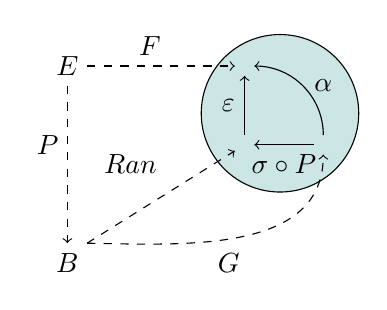
\begin{tikzpicture}
  \def\Xa{0};
   \def\Xm{1.3}
    \def\Xb{2.25};
      \def\Xc{3};
  \def\Yc{2.5};
  \def\Yb{1.75};
  \def\Ya{0};
 
  \node at ( \Xa, \Yc) { $\cat E$ };
  \node at ( \Xa, \Ya) { $\cat B$ };
  \node (1) at (\Xb, \Yc) {};
  \node (2) at (\Xb, \Yb - 0.25) {};
  \node (3) at (\Xb + 1, \Yb - 0.25) {};

  \draw (\Xc - 0.3, \Yc - 0.6)[fill=blue!50!green!20]  ellipse (1 and 1);

  % F
  \node at ( \Xm-0.25, \Yc + 0.25) { $F$ };
  \draw[->, dashed](\Xa + 0.25, \Yc) -- (1);
  % P
  \node at (\Xa - 0.25, \Yb - 0.25) { $P$ };
  \draw[->, dashed](\Xa, \Yc - 0.25) -- (\Xa, \Ya + 0.25);
  % Ran
  \node at (\Xm - 0.5, \Yb - 0.5) { $\text{Ran}$ };
  \draw[->, dashed](\Xa + 0.25, \Ya + 0.25) -- (2);

  % G
  \node at (\Xb - 0.2, \Ya) { $\text{G}$ };
  \draw[->, dashed](\Xa + 0.25, \Ya + 0.25) to [out=-1, in=-90] (3);
  
  \draw[->] (2) -- (1) node[midway, left] {$\varepsilon$};
  \draw[->] (3) -- (2) node[midway, below] {$\sigma \circ P$};
  \draw[->] (3) to [out=90, in=0] (1);
  \node at (\Xb + 1, \Yb + 0.5) {$\alpha$};
\end{tikzpicture}
\]

\begin{exercise}
为 \hask{Ran} 实现 \hask{Functor} 实例。
\end{exercise}

\subsection{作为Kan扩张的极限}
我们之前将极限定义为通用锥体。锥体的定义涉及两个范畴:定义图表形状的索引范畴 $\cat J$,以及目标范畴 $\cat C$。图表是一个将形状嵌入目标范畴的函子 $D \colon \cat J \to \cat C$。

我们可以引入第三个范畴 $\mathbf 1$:这是一个包含单个对象和单个恒等箭头的终端范畴。然后,我们可以使用从该范畴到 $\cat E$ 的函子 $X$ 来选取锥体的顶点 $x$。由于 $\mathbf 1$ 在 $\mathbf{Cat}$ 中是终端的,我们也有从 $\cat J$ 到它的唯一函子,我们称之为 $!$。它将所有对象映射到 $\mathbf 1$ 的唯一对象,并将所有箭头映射到其恒等箭头。

事实证明,$D$ 的极限是图表 $D$ 沿 $!$ 的右Kan扩张。首先,我们观察到复合 $X \circ !$ 将形状 $\cat J$ 映射到单个对象 $x$,因此它起到了常函子 $\Delta_x$ 的作用。因此,它选取了锥体的顶点。以 $x$ 为顶点的锥体是一个自然变换 $\gamma$:
\[
 \begin{tikzcd} [row sep=1cm, column sep=1cm]
 \cat J
 \arrow[rr, "D", "" {name=ID, below} ]
 \arrow[d, bend right, "!"']
 && \cat C
 \\
 \mathbf 1
  \arrow[urr, bend right, "X"']
 \arrow[Rightarrow, "\gamma",  to=ID]
 \end{tikzcd}
\]

以下图表说明了这一点。在左边,我们有两个范畴:$\mathbf 1$ 包含单个对象 $*$,而 $\cat J$ 包含三个对象,形成图表的形状。在右边,我们有 $D$ 的像和 $X \circ !$ 的像,即顶点 $x$。$\gamma$ 的三个分量将顶点 $x$ 连接到图表。$\gamma$ 的自然性确保了形成锥体侧面的三角形交换。

\[
 \begin{tikzcd}
  & *
 \\
\\
1 
\arrow[rr, red]
\arrow[rd, red]
&& 2
\arrow[dl, red]
\\
& 3
 \end{tikzcd}
 \qquad
 \begin{tikzcd}
  & x
\arrow[ddr, "\gamma_2"]
 \arrow[ddl, "\gamma_1"']
 \arrow[ddd, "\gamma_3"]
 \\
\\
D 1 
\arrow[rr, red]
\arrow[rd, red]
&& D 2
\arrow[dl, red]
\\
& D 3
 \end{tikzcd}
 \]

右Kan扩张 $(\text{Ran}_! D, \varepsilon)$ 是通用的这种锥体。$\text{Ran}_! D$ 是一个从 $\mathbf 1$ 到 $\cat C$ 的函子,因此它在 $\cat C$ 中选择一个对象。这确实是通用锥体的顶点,$\text{Lim} D$。

通用性意味着对于任何对 $(X, \gamma)$,存在一个自然变换 $\sigma \colon X \to \text{Ran}_! D$ 
\[
\begin{tikzcd}[row sep=2cm, column sep=2cm]
\cat J  \ar[d, "!"', "" {name=P}]
            \ar[r, "D", ""  {name=F, below, near start, bend right}]
&
\cat C
\\
\mathbf 1
    \ar[ur, bend left, "X", "" {name=G, below}]
    \ar[ur, bend right, "\text{Ran}_! D"', "" {name=Ran}]
\arrow[Rightarrow, "\sigma", from=G, to=Ran]
\end{tikzcd}
\]
它将 $\gamma$ 分解。

变换 $\sigma$ 只有一个分量 $\sigma_*$,它是一个连接顶点 $x$ 到顶点 $\text{Lim} D$ 的箭头 $h$。分解:
 \[ \gamma = \varepsilon \cdot (\sigma \circ !) \]
在分量中表示为:
\[ \gamma_i = \varepsilon_i \circ h \]
它使得以下图表中的三角形交换:
\[
 \begin{tikzcd}[row sep=1cm]
  & x
\arrow[dddl, "\gamma_1"']
\arrow[ddddr, "\gamma_3"]
\arrow[dddrr, "\gamma_2"]
\arrow[dd, dashed, "h"']
 \\
 \\
 & \text{Lim} D
\arrow[dl, blue, "\varepsilon_1"]
\arrow[ddr, blue, "\varepsilon_3"']
\arrow[drr, blue, "\varepsilon_2"]
\\
D 1 
\arrow[rrr, red]
\arrow[rrd, red]
&&& D 2
\arrow[dl, red]
\\
&& D 3
 \end{tikzcd}
 \]
这个通用条件使得 $\text{Lim} D$ 成为图表 $D$ 的极限。

\subsection{左伴随作为右Kan延拓}

我们首先将Kan延拓描述为伴随关系的推广。从图示来看,如果我们有一对伴随函子$L \dashv R$,我们期望左函子是恒等函子沿右函子的右Kan延拓。
\[ L \cong \text{Ran}_R \text{Id} \]
当然,Kan扩展的余单位(counit)与伴随(adjunction)的余单位是相同的:

 \[
 \begin{tikzcd} [row sep=1cm, column sep=1cm]
 \cat C
 \arrow[rr, "\text{Id}", "" {name=ID, below} ]
 \arrow[d, bend right, "R"']
 && \cat C
 \\
 \cat D
  \arrow[urr, bend right, "L"']
 \arrow[Rightarrow, "\varepsilon",  to=ID]
 \end{tikzcd}
\]
我们还需要证明其具有泛性(universality):
\[
 \begin{tikzcd} [row sep=1cm, column sep=1cm]
 \cat C
 \arrow[rr, "\text{\text{Id}}", "" {name=ID, below} ]
 \arrow[d, bend right, "R"']
 && \cat C
 \\
 \cat D
  \arrow[urr, bend right, "G"']
 \arrow[Rightarrow, "\alpha",  to=ID]
 \end{tikzcd}
 \qquad %----%
\begin{tikzcd}[row sep=2cm, column sep=2cm]
\cat C  \ar[d, "R"', "" {name=P}]
            \ar[r, "R", ""  {name=F, below, near start, bend right}]
&
\cat D
\\
\cat D
    \ar[ur, bend left, "G", "" {name=G, below}]
    \ar[ur, bend right, "L"', "" {name=Ran}]
\arrow[Rightarrow, "\sigma", from=G, to=Ran]
\end{tikzcd}
\]
为此,我们可以利用伴随关系的单位:
\[ \eta \colon \text{Id} \to R \circ L \]
我们构造$\sigma$为复合:
\[ G \rightarrow G \circ \text{Id} \xrightarrow{G \circ \eta} G \circ R \circ L \xrightarrow{\alpha \circ L} \text{Id} \circ L \rightarrow L\]
换句话说,我们定义$\sigma$为:
\[ \sigma = (\alpha \circ L) \cdot (G \circ \eta) \]

我们可以提出一个相反的问题:如果$\text{Ran}_R \text{Id}$存在,它是否自动成为$R$的左伴随?事实证明,我们还需要一个额外的条件:Kan延拓必须被$R$保持,即:

\[ R \circ \text{Ran}_R \text{Id} \cong \text{Ran}_R R \]
我们将在下一节中看到,这个条件的右侧定义了余密度单子。

\begin{exercise}
证明分解条件:
\[ \alpha = \varepsilon \cdot (\sigma \circ R) \]
对于上面定义的$\sigma$。提示:绘制相应的弦图并使用伴随关系的三角恒等式。
\end{exercise}

\subsection{余密度单子(Codensity Monad)}

我们已经看到,每一个伴随函子 $L \dashv F$ 都会产生一个单子 $F \circ L$。事实上,这个单子是 $F$ 沿 $F$ 的右 Kan 扩张。有趣的是,即使 $F$ 没有左伴随,Kan 扩张 $\text{Ran}_F F$ 仍然是一个单子,称为\emph{余密度单子},记作 $T^F$:
\[ T^F = \text{Ran}_F F \]

如果我们认真地将 Kan 扩张解释为分数,那么余密度单子将对应于 $F/F$。一个使得这个“分数”等于恒等函子的函子被称为余密(codense)。

为了证明 $T^F$ 是一个单子,我们需要定义单子的单位(unit)和乘法(multiplication):
\[ \eta \colon \text{Id} \to T^F \]
\[ \mu \colon T^F \circ T^F \to  T^F \]
这两者都来自于普遍性。对于每一个 $(G, \alpha)$,我们都有一个 $\sigma$:
\[
 \begin{tikzcd} [row sep=1cm, column sep=1cm]
 \cat D
 \arrow[rr, "F", "" {name=ID, below} ]
 \arrow[d, bend right, "F"']
 && \cat C
 \\
 \cat C
  \arrow[urr, bend right, "G"']
 \arrow[Rightarrow, "\alpha",  to=ID]
 \end{tikzcd}
 \qquad
\begin{tikzcd}[row sep=2cm, column sep=2cm]
\cat D  \ar[d, "F"', "" {name=P}]
            \ar[r, "F", ""  {name=F, below, near start, bend right}]
&
\cat C
\\
\cat C
    \ar[ur, bend left, "G", "" {name=G, below}]
    \ar[ur, bend right, "T^F = \text{Ran}_F F"', "" {name=Ran}]
\arrow[Rightarrow, "\sigma", from=G, to=Ran]
\end{tikzcd}
\]

为了得到单位,我们将 $G$ 替换为恒等函子 $\text{Id}$,并将 $\alpha$ 替换为恒等自然变换。

为了得到乘法,我们将 $G$ 替换为 $T^F \circ T^F$,并注意到我们可以使用 Kan 扩张的余单位(counit):
\[ \varepsilon \colon  T^F \circ F \to F \]
我们可以选择类型为 $\alpha$ 的:
\[ \alpha \colon T^F \circ T^F \circ F \to F \]
并将其定义为复合:
\[ T^F \circ T^F \circ F \xrightarrow{id \circ \varepsilon} T^F \circ F \xrightarrow{\varepsilon} F\]
或者,使用 whiskering 记号:
\[ \alpha = \varepsilon \cdot (T^F \circ \varepsilon) \]
对应的 $\sigma$ 给出了单子的乘法。

现在让我们证明,如果我们从一个伴随开始:
\[ \cat D(L c, d) \cong \cat C (c, F d) \]
那么余密度单子由 $F \circ L$ 给出。让我们从任意函子 $G$ 到 $F \circ L$ 的映射开始:
\[ [\cat C, \cat C](G, F \circ L) \cong  \int_c \cat C (G c, F (L c)) \]
我们可以使用 Yoneda 引理重写它:
\[ \cong \int_c \int_d \Set\big(\cat D(L c, d), \cat C (G c, F d)\big) \]
在这里,对 $d$ 取 end 的效果是将 $d$ 替换为 $L c$。我们现在可以使用伴随:
\[ \cong \int_c \int_d \Set\big(\cat C(c, F d), \cat C (G c, F d)\big) \]
并对 $c$ 进行 ninja-Yoneda 积分,得到:
\[ \cong \int_d \cat C (G (F d), F d) \]
这反过来定义了一组自然变换:
\[ \cong [\cat D, \cat C](G \circ F, F) \]
通过 $F$ 的前复合是右 Kan 扩张的左伴随:
\[ [\cat D, \cat C](G \circ F, F) \cong  [\cat C, \cat C] (G, \text{Ran}_F F)\]
由于 $G$ 是任意的,我们得出结论:$F \circ L$ 确实是余密度单子 $\text{Ran}_F F$。

由于每一个单子都可以从某个伴随导出,因此可以得出\emph{每一个单子都是某个伴随的余密度单子}。

\subsection{Haskell 中的密度单子}

将密度单子(codensity monad)翻译到 Haskell 中,我们得到:
\begin{haskell}
newtype Codensity f c = C (forall d. (c -> f d) -> f d)
\end{haskell}
以及提取器:
\begin{haskell}
runCodensity :: Codensity f c -> forall d. (c -> f d) -> f d
runCodensity (C h) = h
\end{haskell}
这看起来非常类似于延续单子(continuation monad)。事实上,如果我们选择 \hask{f} 为恒等函子(identity functor),它就会变成延续单子。我们可以将 \hask{Codensity} 视为接受一个回调函数 \hask{(c -> f d)},并在类型为 \hask{c} 的结果可用时调用它。

以下是单子实例:
\begin{haskell}
instance Monad (Codensity f) where
  return x = C (\k -> k x)
  m >>= kl = C (\k -> runCodensity m (\a -> runCodensity (kl a) k))
\end{haskell}
同样,这几乎与延续单子完全相同:
\begin{haskell}
instance Monad (Cont r) where
  return x = Cont (\k -> k x)
  m >>= kl = Cont (\k -> runCont m (\a -> runCont (kl a) k))
\end{haskell}
这就是为什么 \hask{Codensity} 具有延续传递风格(continuation passing style)的性能优势。由于它以“由内向外”的方式嵌套延续,因此可以用于优化由 \hask{do} 块生成的绑定长链。

这一特性在处理自由单子(free monads)时尤为重要,自由单子会在树状结构中累积绑定。当我们最终解释自由单子时,这些累积的绑定需要遍历不断增长的树。对于每个绑定,遍历都从根节点开始。将此与之前反转列表的示例进行比较,后者通过将函数累积在 FIFO 队列中进行了优化。密度单子提供了相同类型的性能改进。

\begin{exercise}
为 \hask{Codensity} 实现 \hask{Functor} 实例。
\end{exercise}
\begin{exercise}
为 \hask{Codensity} 实现 \hask{Applicative} 实例。
\end{exercise}

\section{左 Kan 扩展}

正如右 Kan 扩展被定义为函子预组合的\emph{右}伴随,左 Kan 扩展被定义为函子预组合的\emph{左}伴随:
\[ [\cat B, \cat C](\text{Lan}_P F , G) \cong  [\cat E, \cat C] (F, G \circ P) \]
(还有\emph{后}组合的伴随:它们被称为 Kan 提升。)

或者,$\text{Lan}_P F$ 可以定义为一个配备有称为单位(unit)的自然变换的函子:
\[ \eta \colon F \to \text{Lan}_P F \circ P \]
\[
 \begin{tikzcd} [row sep=1cm, column sep=1cm]
 \cat E
 \arrow[rr, "F", "" {name=ID, below} ]
 \arrow[d, bend right, "P"']
 && \cat C
 \\
 \cat B
  \arrow[urr, blue, bend right, "\text{Lan}_P F"']
 \arrow[Rightarrow, blue, "\eta",  from=ID]
 \end{tikzcd}
\]
注意,左 Kan 扩展的单位方向与右 Kan 扩展的余单位(counit)方向相反。

$(\text{Lan}_P F, \eta)$ 这对是普遍的,意味着对于任何其他对 $(G, \alpha)$,其中
\[ \alpha \colon F \to G \circ P\] 
\[
 \begin{tikzcd} [row sep=1cm, column sep=1cm]
 \cat E
 \arrow[rr, "F", "" {name=ID, below} ]
 \arrow[d, bend right, "P"']
 && \cat C
 \\
 \cat B
  \arrow[urr, red, bend right, "G"']
 \arrow[Rightarrow, red, "\alpha",  from=ID]
 \end{tikzcd}
\]
存在唯一的映射 $\sigma \colon \text{Lan}_P F \to G$ 
\[
\begin{tikzcd}[row sep=2cm, column sep=2cm]
\cat E  \ar[d, "P"', "" {name=P}]
            \ar[r, "F", ""  {name=F, below, near start, bend right}]
&
\cat C
\\
\cat B
    \ar[ur, red, bend left, "G", "" {name=G, below}]
    \ar[ur, blue, bend right, "\text{Lan}_P F"', "" {name=Lan}]
\arrow[Rightarrow, "\sigma", from=Lan, to=G]
\end{tikzcd}
\]
使得 $\alpha$ 被分解为:
\[ \alpha = (\sigma \circ P) \cdot \eta \]
同样,$\sigma$ 的方向与右 Kan 扩展相反。

使用弦图(string diagrams),我们可以将普遍条件描绘为:
\[
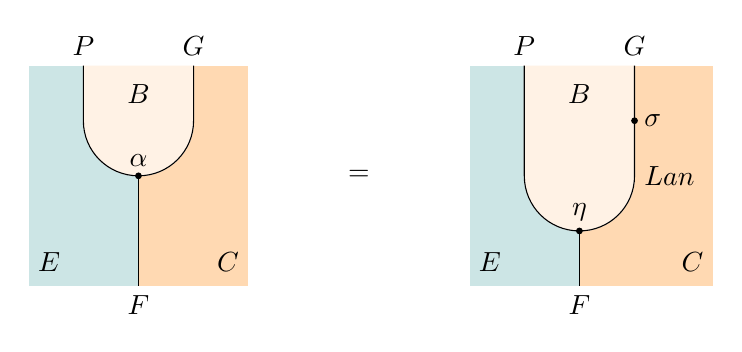
\begin{tikzpicture}
\def \dx {0.7}
\def \dy {-0.7}

\def \xa{-3 * \dx};
\def \xb{-2 * \dx};
\def \xc{-1 * \dx};
\def \xd{0};
\def \xe{1 * \dx};

\def \ya{0};
\def \yb{1 * \dy};
\def \yc{2 * \dy};
\def \yd{3 * \dy};
\def \ye{4 * \dy};

% left background
\filldraw[fill=blue!50!green!20, draw=white] (\xa, \ye) rectangle (\xc, \ya);
% right background
\filldraw[fill=orange!30, draw=white] (\xc, \ye) rectangle (\xe, \ya);
% fill shape\yb
\path [fill=orange!10, draw=white]  (\xb, \ya) to (\xb, \yb) to [out=270, in=180]  (\xc, \yc) to  [out=0, in=270] (\xd, \yb) to (\xd, \ya);

% cup
\draw (\xb, \ya) to (\xb, \yb) to [out=270, in=180]  (\xc, \yc) to  [out=0, in=270] (\xd, \yb) to (\xd, \ya);
\draw (\xc, \yc) -- (\xc, \ye);

% natural transformations
\filldraw[black] (\xc, \yc) circle (1 pt);
\node [above] at (\xc, \yc) {$\alpha$};

% categories
\node[right] at (\xa, \ye + 0.3) {$\cat E$};
\node[left] at (\xe, \ye + 0.3) {$\cat C$};
\node[above] at (\xc, \ya - 0.6) {$\cat B$};
% functors
\node [above] at (\xb, \ya) {$P$};
\node [above] at (\xd, \ya) {$G$};
\node [below] at (\xc, \ye) {$F$};

%-----------------
\node (eq) at (3 * \dx, \yc) {$=$};
% right diagram

\def \xa{5 * \dx};
\def \xb{6 * \dx};
\def \xc{7 * \dx};
\def \xd{8 * \dx};
\def \xe{9 * \dx + 0.3};

% left background
\filldraw[fill=blue!50!green!20, draw=white] (\xa, \ye) rectangle (\xc, \ya);
% right background
\filldraw[fill=orange!30, draw=white] (\xc, \ye) rectangle (\xe, \ya);
% fill shape
\path [fill=orange!10, draw=white]  (\xb, \ya) to (\xb, \yc) to [out=270, in=180]  (\xc, \yd) to  [out=0, in=270] (\xd, \yc) to (\xd, \ya);

% cup
\draw (\xb, \ya) to (\xb, \yc) to [out=270, in=180]  (\xc, \yd) to  [out=0, in=270] (\xd, \yc) to (\xd, \ya);
\draw (\xc, \yd) -- (\xc, \ye);

% natural transformations
\filldraw[black] (\xc, \yd) circle (1 pt);
\node [above] at (\xc, \yd) {$\eta$};

\filldraw[black] (\xd, \yb) circle (1 pt);
\node [right] at (\xd, \yb) {$\sigma$};

% categories
\node[right] at (\xa, \ye + 0.3) {$\cat E$};
\node[left] at (\xe, \ye + 0.3) {$\cat C$};
\node[above] at (\xc, \ya - 0.6) {$\cat B$};
% functors
\node [above] at (\xb, \ya) {$P$};
\node [above] at (\xd, \ya) {$G$};
\node [below] at (\xc, \ye) {$F$};
\node [right] at (\xd, \yc) {$\text{Lan}$};

\end{tikzpicture}
\]

这建立了两个自然变换集合之间的一一对应关系。对于左边的每个 $\alpha$,右边都有一个唯一的 $\sigma$:
\[  [\cat E, \cat C] (F, G \circ P) \cong [\cat B, \cat C](\text{Lan}_P F , G)  \]

\subsection{左Kan扩张作为余端}

回顾忍者余Yoneda引理。对于每一个余预层$F$,我们有:
\[ F b \cong \int^{c} \cat B(c, b) \times F c \]
左Kan扩张将这个公式推广为:
\[ (\text{Lan}_P F)\, b \cong \int^{e} \cat B (P e, b) \times F e \]
对于一个一般的函子$F \colon \cat E \to \cat C$,我们用\index{余幂}余幂代替乘积:
\[ (\text{Lan}_P F)\, b \cong \int^{e} \cat B(P e, b) \cdot F e \]

只要所讨论的余端存在,我们就可以通过考虑映射到某个函子$G$来证明这个公式。我们将自然变换的集合表示为关于$b$的端:
\[\int_b \cat C \big(\int^e \cat B(P e, b) \cdot F e, G b\big) \]
利用余连续性,我们将余端拉出,将其转化为端:
\[\int_b \int_e \cat C \big(\cat B(P e, b) \cdot F e, G b\big) \]
然后我们代入余幂的定义:
\[\int_b \int_e \cat C \big(\cat B(P e, b), \cat C (F e, G b)\big) \]
现在我们可以使用Yoneda引理对$b$进行积分,将$b$替换为$P e$:
\[\int_e \cat C (F e, G (P e))\big) \cong  [\cat E, \cat C] (F, G \circ P) \]
这确实给出了函子预组合的左伴随:
\[ [\cat B, \cat C](\text{Lan}_P F , G) \cong  [\cat E, \cat C] (F, G \circ P) \]

在$\Set$中,余幂退化为笛卡尔积,因此我们得到一个更简单的公式:
\[ (\text{Lan}_P F)\, b \cong \int^{e} \cat B (P e, b) \times F e \]

注意,如果函子$P$有一个右伴随,我们称之为$P^{-1}$:
\[ \cat B(P e , b) \cong \cat E(e, P^{-1} b) \]
我们可以使用忍者余Yoneda引理得到:
\[  (\text{Lan}_P F)\, b \cong (F \circ P^{-1}) b \]
这进一步强化了Kan扩张反转$P$并随后应用$F$的直觉。

\subsection{Haskell 中的左 Kan 扩展}

将左 Kan 扩展的公式翻译到 Haskell 时,我们用存在类型(existential type)替换了余端(coend)。符号表示如下:
\begin{haskell}
type Lan p f b = exists e. (p e -> b, f e)
\end{haskell}
这是我们使用 \hask{GADT} 编码存在类型的方式:
\begin{haskell}
data Lan p f b where
    Lan :: (p e -> b) -> f e -> Lan p f b
\end{haskell}

左 Kan 扩展的单位(unit)是一个从函子 \hask{f} 到 \hask{(Lan p f)} 与 \hask{p} 的复合的自然变换:
\begin{haskell}
unit :: forall p f e'. 
    f e' -> Lan p f (p e')
\end{haskell}
为了实现单位,我们从类型为 \hask{(f e')} 的值开始。我们需要找到某个类型 \hask{e}、一个函数 \hask{p e -> p e'} 以及一个类型为 \hask{(f e)} 的值。显然的选择是取 \hask{e = e'} 并在 \hask{(p e')} 上使用恒等函数:
\begin{haskell}
unit fe = Lan id fe 
\end{haskell}

左 Kan 扩展的计算能力在于其泛性质(universal property)。给定一个函子 \hask{g} 以及一个从 \hask{f} 到 \hask{g} 与 \hask{p} 的复合的自然变换:
\begin{haskell}
type Alpha p f g = forall e. f e -> g (p e)
\end{haskell}
存在一个唯一的自然变换 $\sigma$,从相应的左 Kan 扩展到 \hask{g}:
\begin{haskell}
sigma :: Functor g => Alpha p f g -> forall b. (Lan p f b -> g b)
sigma alpha (Lan pe_b fe) = fmap pe_b (alpha fe)
\end{haskell}
该变换通过单位 $\eta$ 将 $\alpha$ 分解:
\[ \alpha = (\sigma \circ P) \cdot \eta \]
$\sigma$ 的 whiskering 意味着在 \hask{b = p e} 处实例化它,因此 $\alpha$ 的分解实现如下:
\begin{haskell}
factorize :: Functor g => Alpha p f g -> f e -> g (p e)
factorize alpha = sigma alpha . unit
\end{haskell}
\begin{exercise}
为 \hask{Lan} 实现 \hask{Functor} 实例。
\end{exercise}

\subsection{余极限作为Kan扩张}

正如极限可以定义为右Kan扩张一样,余极限也可以定义为左Kan扩张。

我们从一个索引范畴$\cat J$开始,它定义了余极限的形状。函子$D$在目标范畴$\cat C$中选择这个形状。余锥的顶点由一个从终对象单对象范畴$\Cat 1$出发的函子选择。自然变换定义了一个从$D$到$X$的余锥:
\[
 \begin{tikzcd} [row sep=1cm, column sep=1cm]
 \cat J
 \arrow[rr, "D", "" {name=ID, below} ]
 \arrow[d, bend right, "!"']
 && \cat C
 \\
 \Cat 1
  \arrow[urr, bend right, "X"']
 \arrow[Rightarrow, "\gamma",  from=ID]
 \end{tikzcd}
\]

这里是一个由三个对象和三个态射(不包括恒等态射)组成的简单形状的示例。对象$x$是函子$X$下单对象$*$的像:
\[
 \begin{tikzcd}
1 
\arrow[rr, red]
\arrow[rd, red]
&& 2
\arrow[dl, red]
\\
& 3
\\
\\
& *
 \end{tikzcd}
 \qquad
 \begin{tikzcd}
D 1 
\arrow[rr, red]
\arrow[rd, red]
\arrow[dddr, "\gamma_1"']
&& D 2
\arrow[dl, red]
\arrow[dddl, "\gamma_2"]
\\
& D 3
\arrow[dd, "\gamma_3"]
\\
\\
&x
 \end{tikzcd}
 \]
余极限是通用余锥,它由$D$沿函子$!$的左Kan扩张给出:
\[ \text{Colim}\; D = \text{Lan}_! D \]

\subsection{右伴随作为左Kan扩张}

我们已经看到,当我们有一个伴随 $L \vdash R$ 时,左伴随与右Kan扩张相关。对偶地,如果右伴随存在,它可以表示为恒等函子的左Kan扩张:
\[ R \cong \text{Lan}_L \text{Id} \]
反之,如果恒等函子的左Kan扩张存在并且它保持函子 $L$:
\[ L \circ \text{Lan}_L \text{Id} \cong \text{Lan}_L L \]
那么 $\text{Lan}_L \text{Id}$ 就是 $L$ 的右伴随。$L$ 沿自身的左Kan扩张称为\index{密度余单子}密度余单子。

Kan扩张的单位与伴随的单位相同:
\[
 \begin{tikzcd} [row sep=1cm, column sep=1cm]
 \cat C
 \arrow[rr, "\text{Id}", "" {name=ID, below} ]
 \arrow[d, bend right, "L"']
 && \cat C
 \\
 \cat D
  \arrow[urr, bend right, "R"']
 \arrow[Rightarrow, "\eta",  from=ID]
 \end{tikzcd}
\]
普遍性的证明与右Kan扩张的证明类似。

\begin{exercise}
为密度余单子实现 \hask{Comonad} 实例:
\begin{haskell}
data Density f c where
   D :: (f d -> c) -> f d -> Density f c
\end{haskell}
\end{exercise}

\subsection{Day 卷积作为 Kan 扩张}

我们已经看到 Day 卷积被定义为在幺半范畴 $\cat C$ 上的余预层范畴中的张量积:
\[ (F \star G) c = \int^{a, b} \cat C (a \otimes b, c) \times F a \times G b \]
余预层,即 $[\cat C, \Set]$ 中的函子,也可以使用\index{外部张量积}\emph{外部张量积}进行张量积。两个对象的外部积不是在同一个范畴中生成一个对象,而是在另一个范畴中选择一个对象。在我们的例子中,两个函子的积最终落在 $\cat C \times \cat C$ 上的余预层范畴中:
\[ \bar{\otimes} \colon [\cat C, \Set] \times [\cat C, \Set] \to [\cat C \times \cat C, \Set] \]
两个余预层在 $\cat C \times \cat C$ 中的一对对象上的积由以下公式给出:
\[ (F \bar{\otimes} G)\langle a, b \rangle = F a \times G b \]

事实证明,两个函子的 Day 卷积可以表示为它们的外部积在 $\cat C$ 中的张量积下的左 Kan 扩张:
\[ F \star G \cong \text{Lan}_{\otimes} (F \bar{ \otimes } G) \]
图示如下:
\[
 \begin{tikzcd} [row sep=1cm, column sep=1cm]
 \cat C \times \cat C
 \arrow[rr, "F \bar{\otimes} G", "" {name=ID, below} ]
 \arrow[d, bend right, "\otimes"']
 && \Set
 \\
 \cat C
  \arrow[urr, bend right, "\text{Lan}_{\otimes} (F \bar{ \otimes } G)"']
 \end{tikzcd}
\]

确实,使用左 Kan 扩张的余积公式,我们得到:
\[ (\text{Lan}_{\otimes} (F \bar{ \otimes } G)) c \cong \int^{\langle a, b\rangle} \cat C ( a \otimes b, c) \cdot (F \bar{ \otimes } G)\langle a, b\rangle\]

\[ \cong \int^{\langle a, b\rangle} \cat C ( a \otimes b, c) \cdot (F a \times G  b) \]
由于这两个函子是 $\Set$ 值的,余幂退化为笛卡尔积:
\[ \cong \int^{\langle a, b\rangle} \cat C ( a \otimes b, c) \times F a \times G  b \]
并重现了 Day 卷积的公式。

\section{常用公式}
\begin{itemize}
\item 余幂:
\[ \cat C (A \cdot b, c) \cong \Set \big( A, \cat C (b, c)\big) \]
\item 幂:
\[ \cat C (b, A \pitchfork c) \cong \Set  \big(A, \cat C(b, c)\big) \]
\item 右 Kan 扩张:
\[ [\cat E, \cat C](G \circ P, F) \cong [\cat B, \cat C](G, \text{Ran}_P F) \]
 \[ (\text{Ran}_P F) b \cong \int_e \cat B (b, P e) \pitchfork F e \]
\item 左 Kan 扩张:
\[ [\cat B, \cat C](\text{Lan}_P F , G) \cong  [\cat E, \cat C] (F, G \circ P) \]
\[ (\text{Lan}_P F)\, b \cong \int^{e} \cat B(P e, b) \cdot F e \]
\item $\Set$ 中的右 Kan 扩张:
  \[ (\text{Ran}_P F) b \cong \int_e \Set \big( \cat B (b, P e), F e\big) \]
\item $\Set$ 中的左 Kan 扩张:
\[ (\text{Lan}_P F) b \cong \int^{e} \cat B (P e, b) \times F e \]


\end{itemize}


\end{document}
